\documentclass[10pt,twocolumn]{article}
\usepackage[margin=0.75in, top=0.7in, bottom=0.7in]{geometry}
\usepackage{graphicx}
\usepackage{booktabs}
\usepackage{amsmath}
\usepackage{caption}
\usepackage{subcaption}
\usepackage{hyperref}
\usepackage{parskip}
\usepackage{titlesec}
\usepackage{enumitem}
\usepackage{microtype}

\titlespacing{\section}{0pt}{6pt}{3pt}
\titlespacing{\subsection}{0pt}{4pt}{2pt}
\captionsetup{font=small, labelfont=bf, skip=4pt}
\setlist{noitemsep, topsep=2pt}

\title{\textbf{Resting-State Functional Connectivity and Predictive Modeling of Fluid Intelligence Across the Adult Lifespan}\\[4pt]
\large{Human Brain Mapping -- Assignment 2}}
\author{Arya}
\date{}

\begin{document}
\maketitle
\vspace{-10pt}

% ============================================================
\section{Part 1: Parcellation and Connectivity}
% ============================================================

\subsection{Time-Series Extraction}

The HCP resting-state CIFTI file (\texttt{rfMRI\_REST1\_LR\_Atlas\_hp2000\_clean}) contains 1200 timepoints across 91,282 grayordinates (TR = 0.72\,s, ~14.4 min). The Schaefer 400-parcel, 17-network atlas was applied by mapping cortical surface vertex indices from the atlas to the corresponding positions in the dtseries. Of the 91,282 grayordinates, 58,606 (64.2\%) were assigned to a parcel; the remainder are subcortical structures not covered by this cortical-only atlas, which is expected. Mean BOLD signal per parcel yielded a 400$\times$1200 matrix.

\subsection{Time-Series Observations}

Figure~\ref{fig:timeseries} shows z-scored BOLD signals for 20 representative parcels, one per network community. Several patterns stand out. Primary visual parcels (VisCent, VisPeri) show smoother, lower-variance traces compared to association areas. Default Mode parcels display slower, higher-amplitude oscillations with more prominent low-frequency content. Limbic parcels are notably noisier, likely reflecting susceptibility artifacts in orbitofrontal regions. Despite these differences, all parcels share the characteristic resting-state infra-slow oscillatory structure (0.01--0.1\,Hz).

\begin{figure}[h]
    \centering
    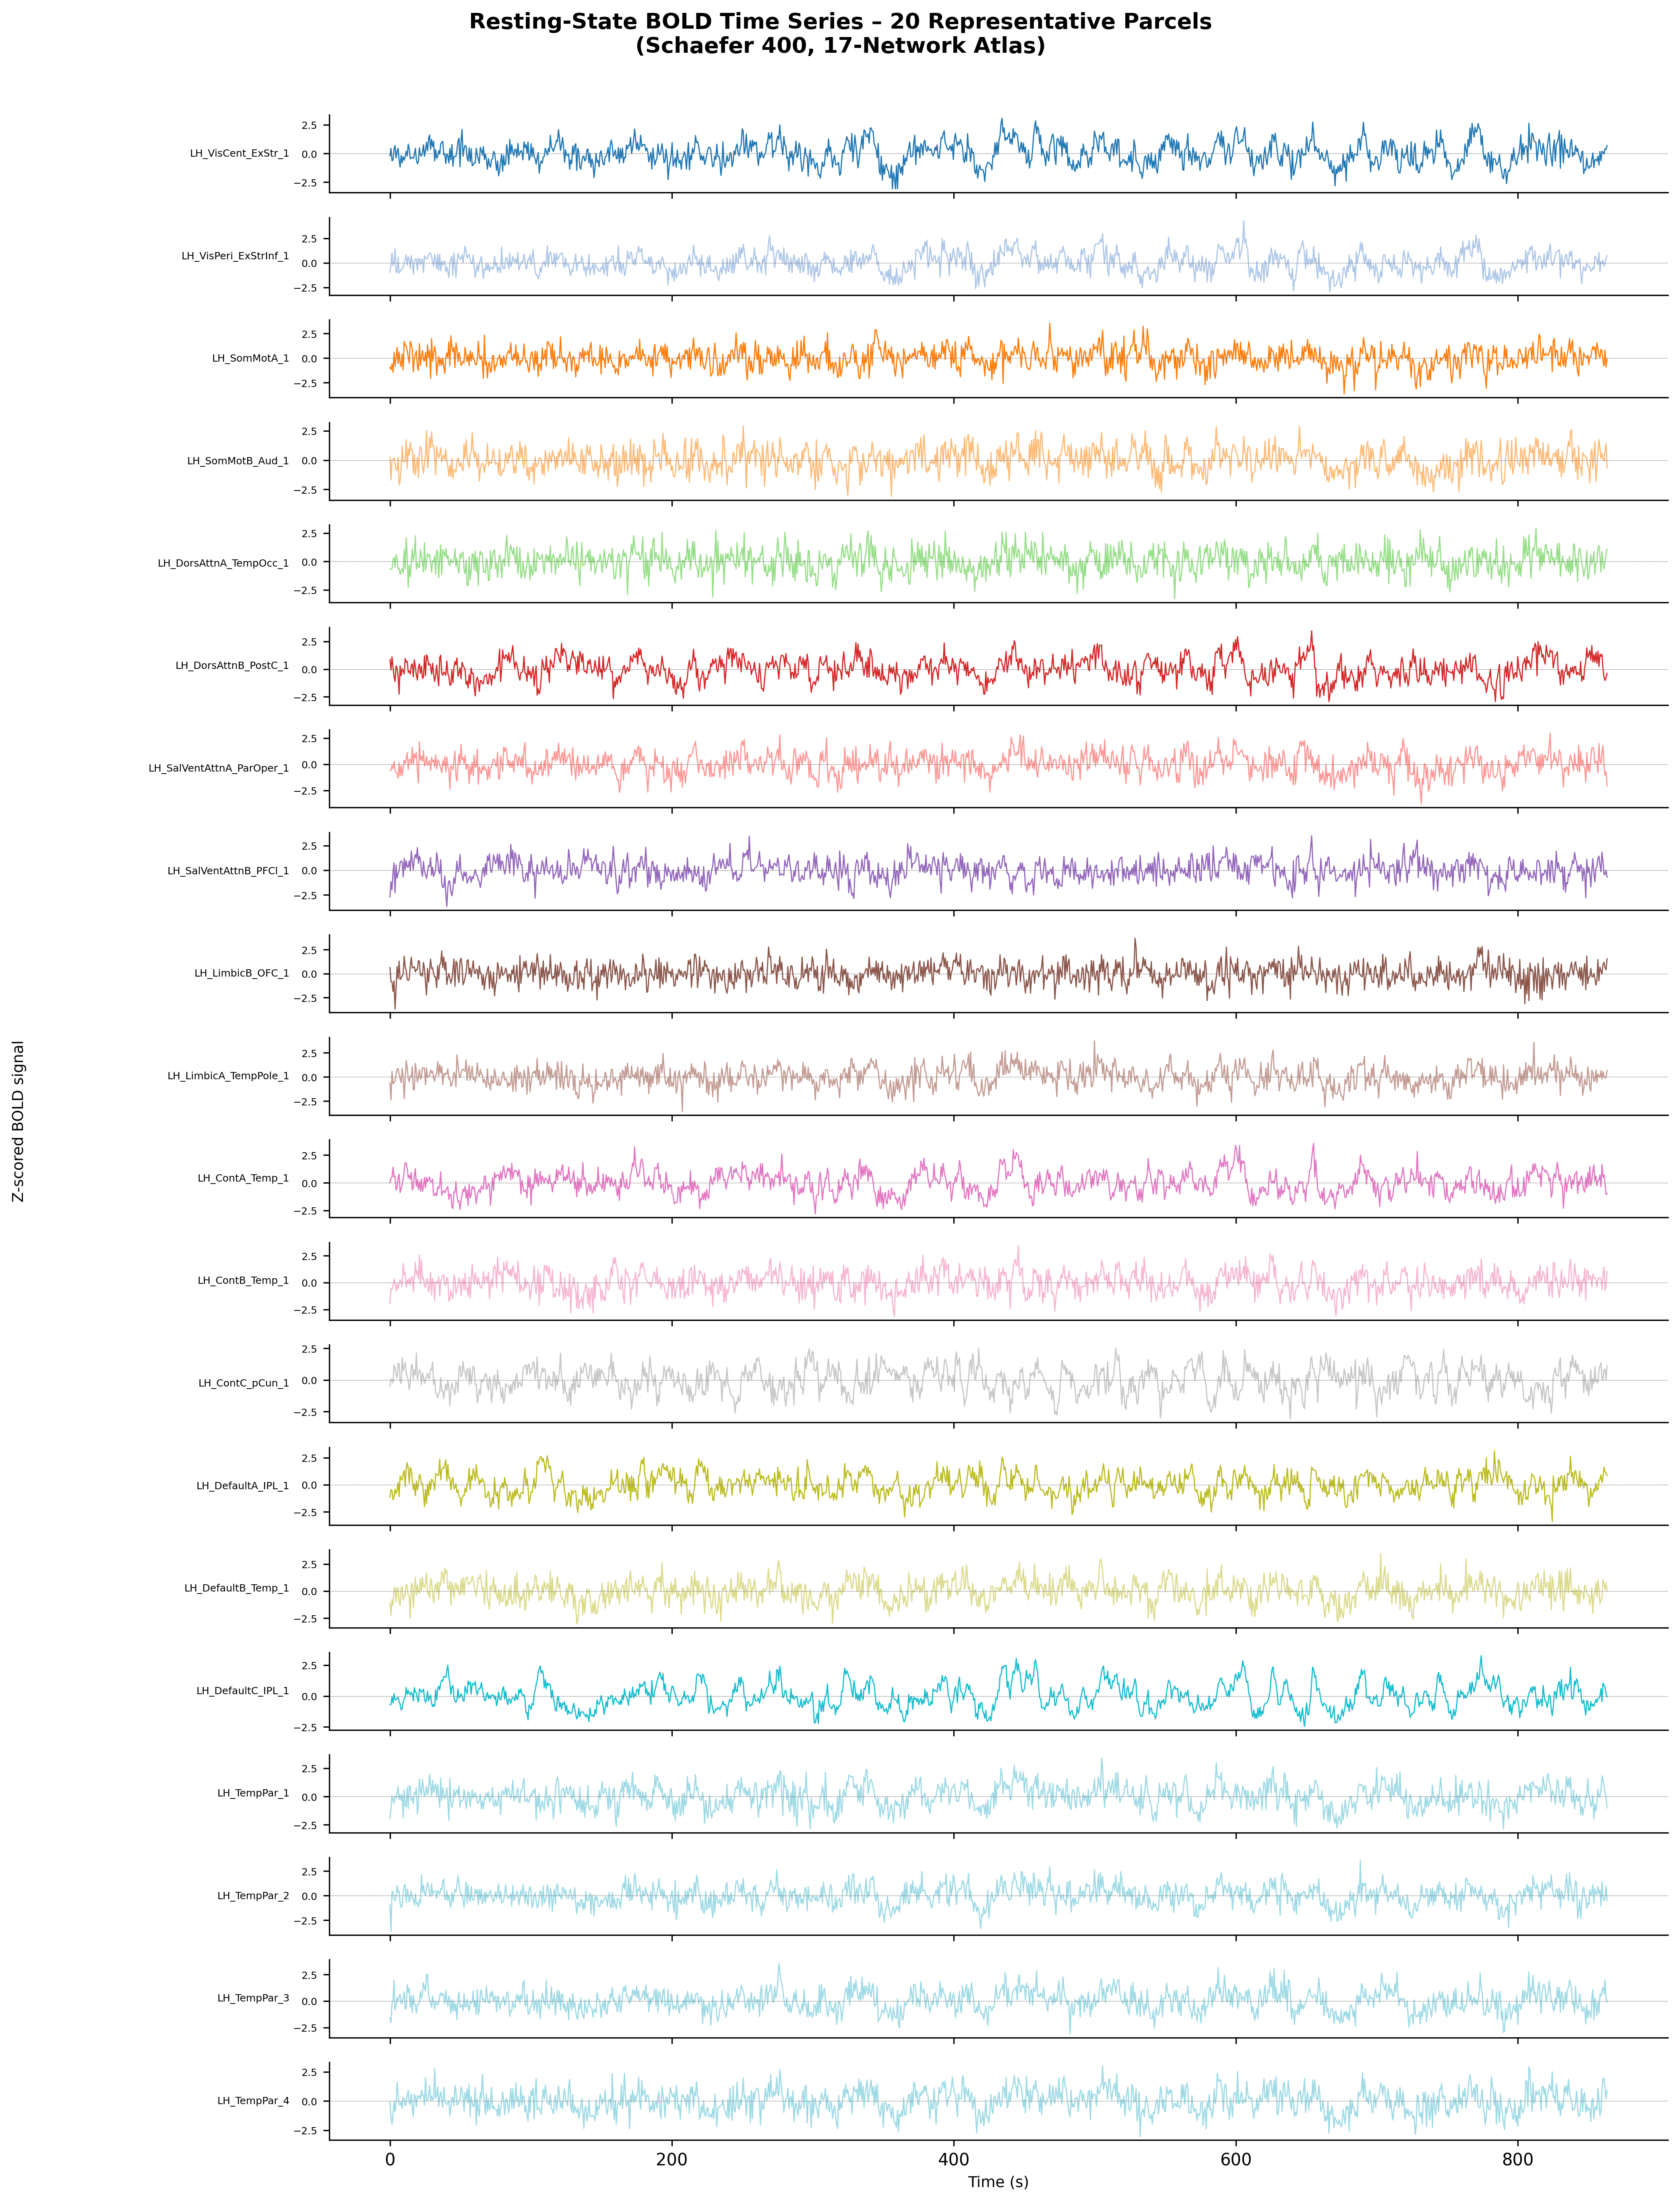
\includegraphics[width=\linewidth]{figures/timeseries_20rois.png}
    \caption{Z-scored BOLD time series for 20 representative Schaefer parcels, one per 17-network community. Each trace is color-coded by network.}
    \label{fig:timeseries}
\end{figure}

\subsection{Functional Connectivity Matrices}

The 400$\times$400 Pearson correlation matrix (Figure~\ref{fig:matrices}) shows clear modular block structure with parcels ordered by network. Within-network blocks are strongly positive (dark red), particularly for Visual (r $\approx$ 0.6--0.9), Somatomotor, and Default Mode networks. Between-network anticorrelation (blue) is visible between Visual/Somatomotor and Default Mode regions, reproducing the canonical task-positive vs. task-negative organization first described by Fox et al. (2005). The r range of $[-0.45,\,1.00]$ indicates a broad but physiologically reasonable connectivity profile for a single subject.

The Fisher z-transformed matrix shares identical structure but with enhanced contrast at high correlation values (z range: $[-0.48,\,1.38]$). This transformation linearizes the relationship between r and variance, making the matrix more appropriate for statistical inference. Network boundaries become visually sharper in z-space, and the Default Mode blocks in particular appear more prominent. Both matrices confirm the expected hierarchical organization: primary sensory cortices form compact, isolated clusters, while association networks (Default, Control, Salience) show broader cross-network coupling.

\begin{figure}[h]
    \centering
    \begin{subfigure}[b]{0.49\linewidth}
        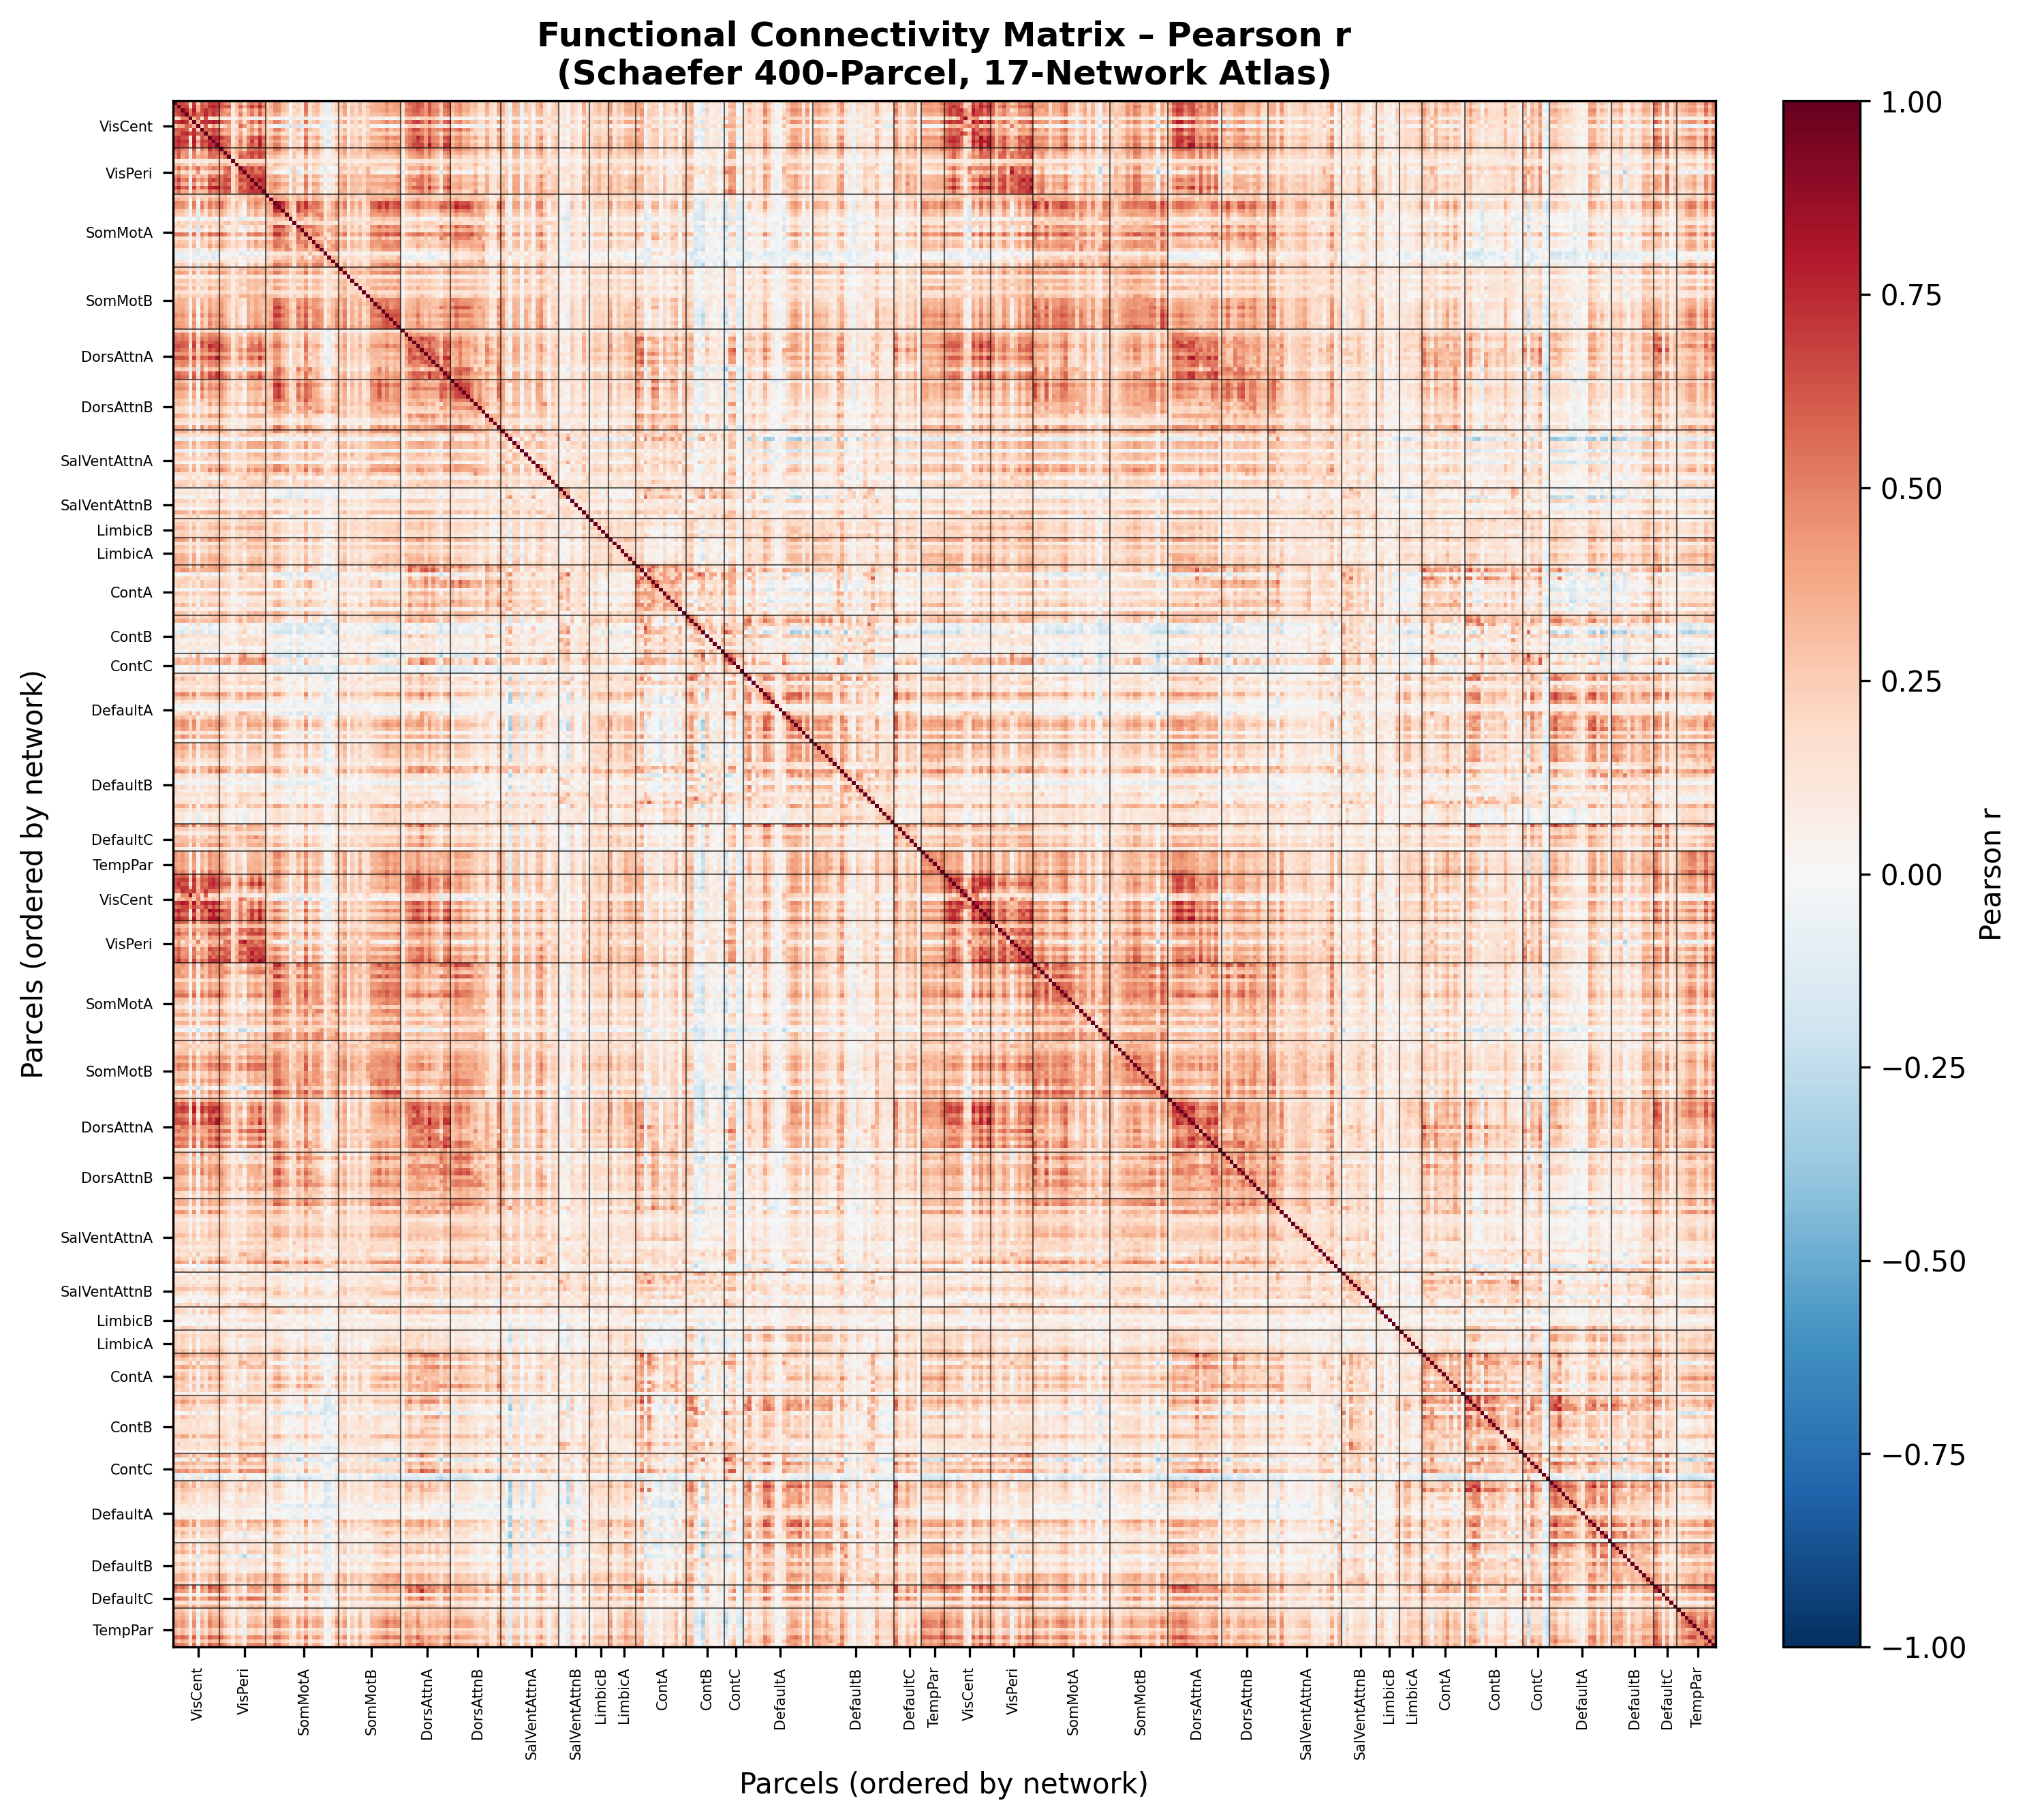
\includegraphics[width=\linewidth]{figures/heatmap_pearson.png}
        \caption{Pearson r}
    \end{subfigure}
    \hfill
    \begin{subfigure}[b]{0.49\linewidth}
        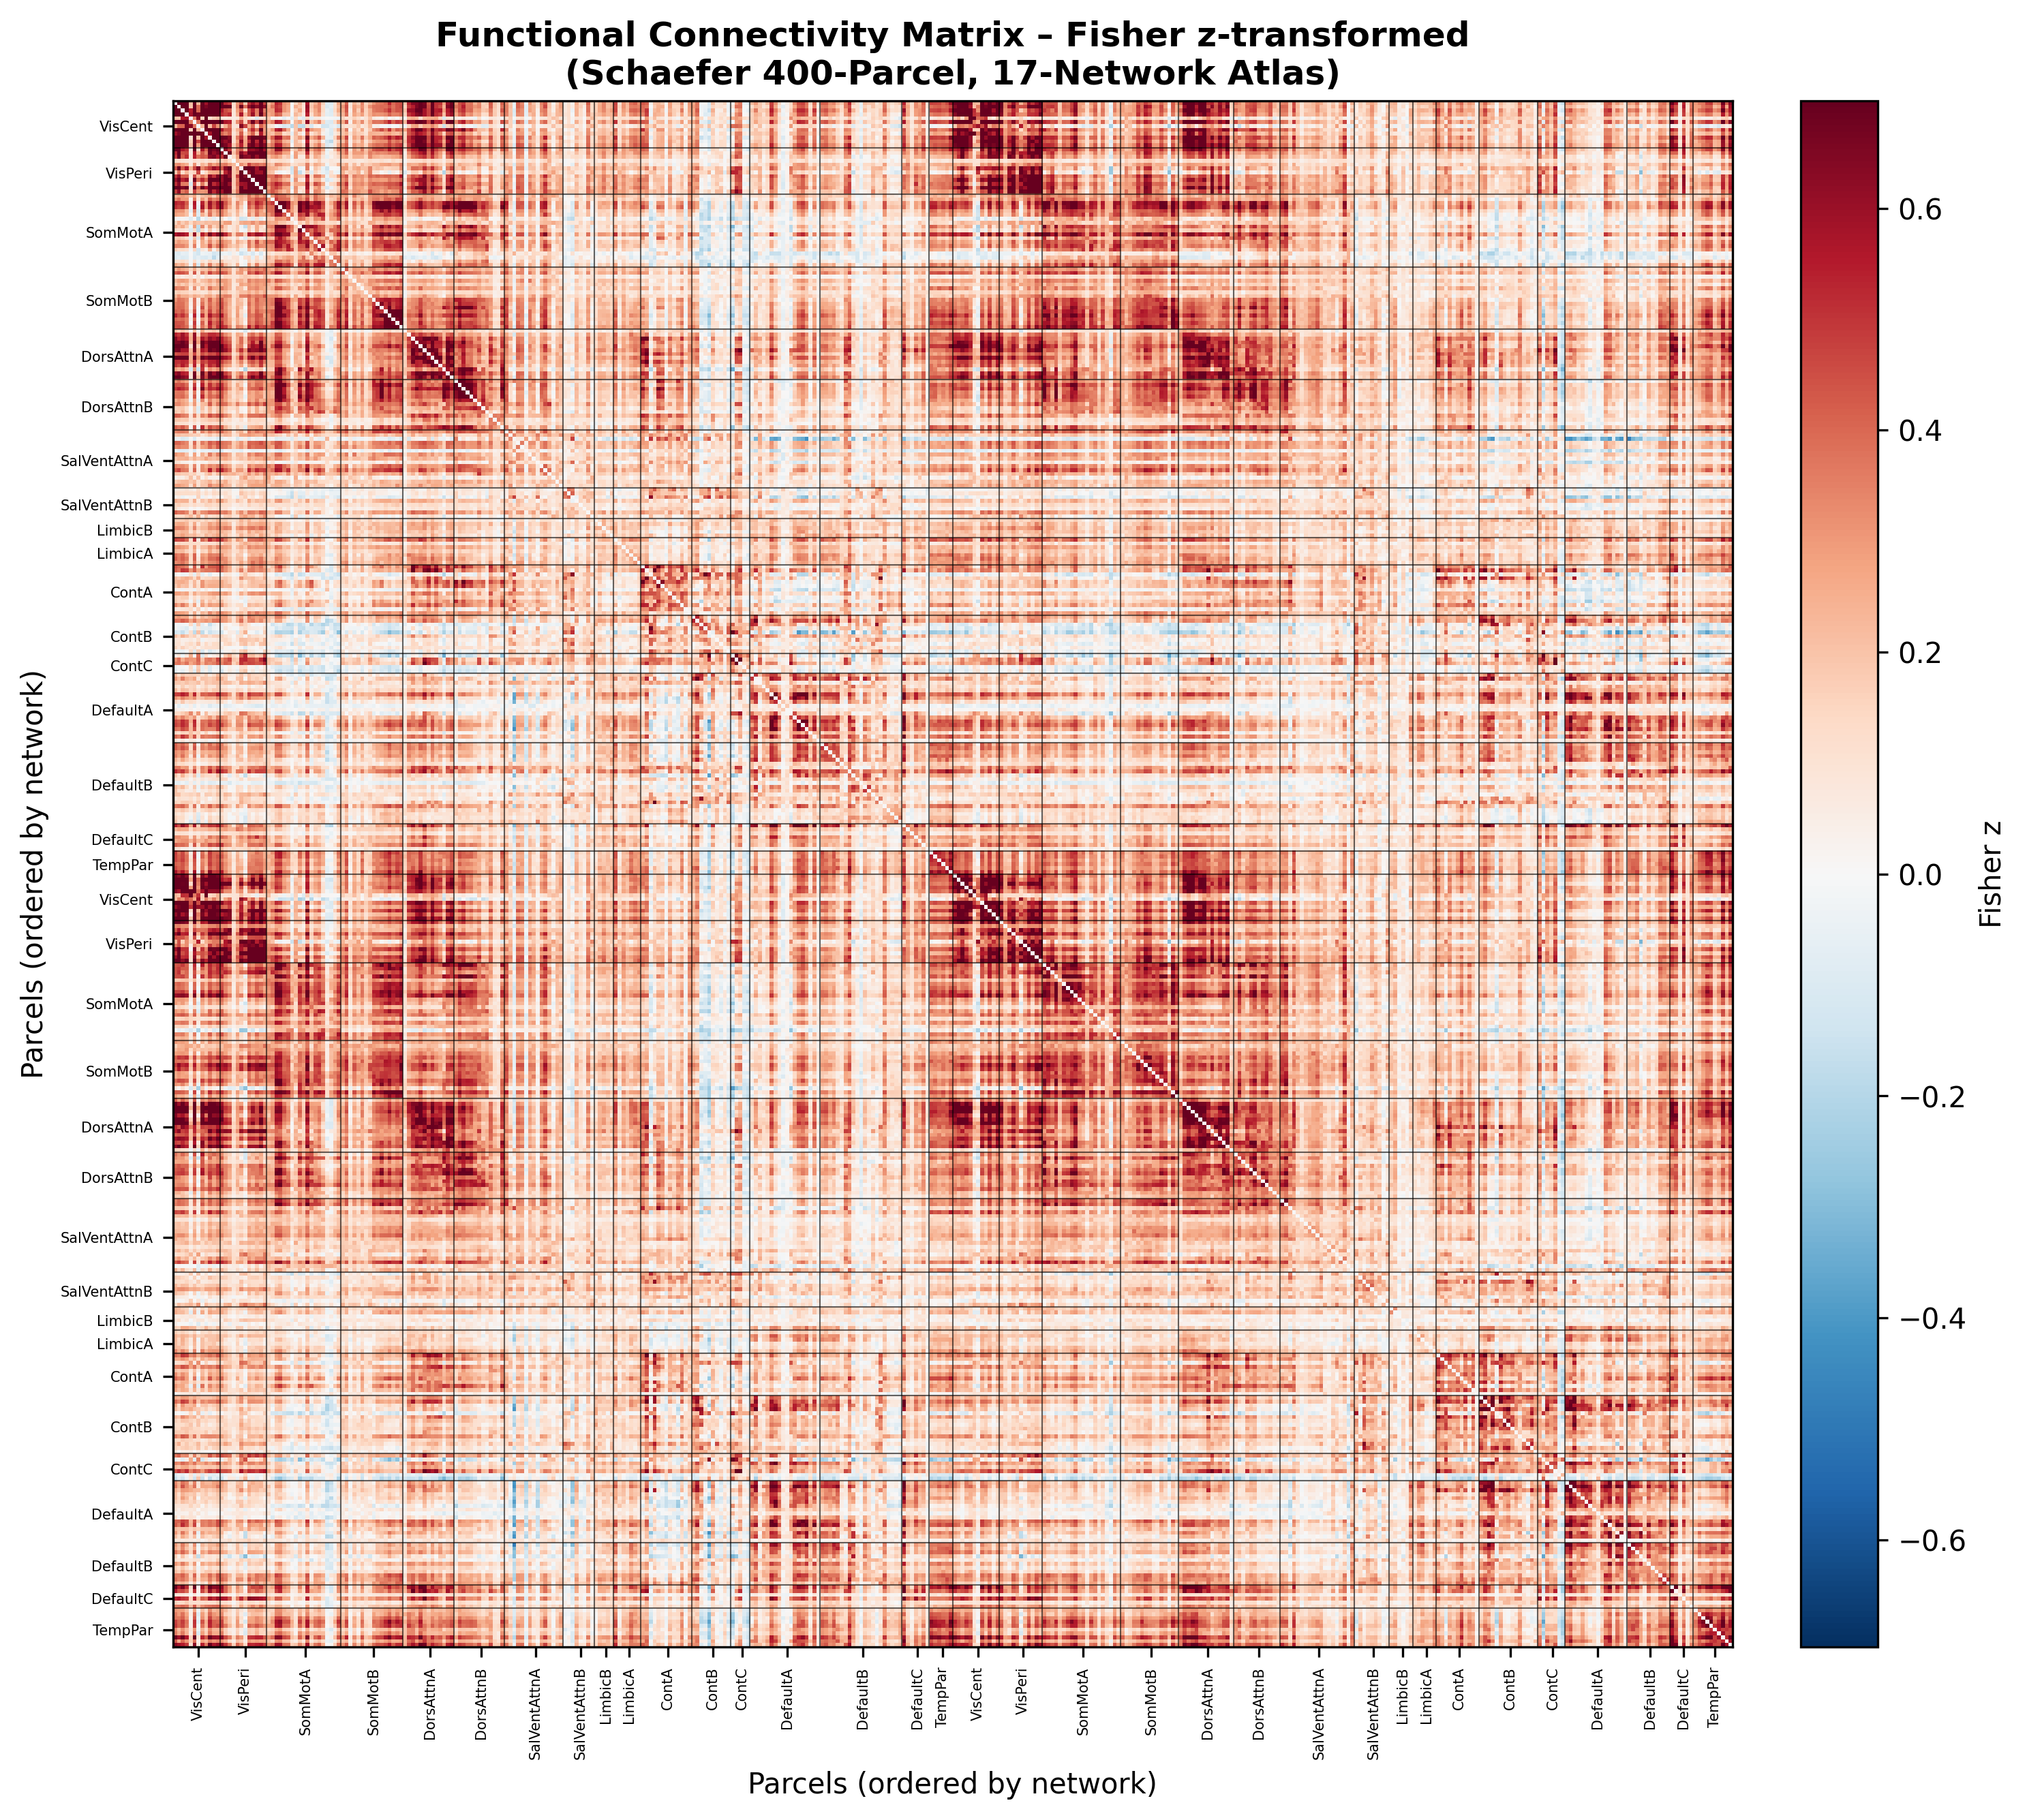
\includegraphics[width=\linewidth]{figures/heatmap_fisherz.png}
        \caption{Fisher z}
    \end{subfigure}
    \caption{400$\times$400 functional connectivity matrices for the single HCP subject (Schaefer atlas). Parcels ordered by 17-network assignment; black lines indicate network boundaries.}
    \label{fig:matrices}
\end{figure}

% ============================================================
\section{Part 2: Lifespan Connectivity Analysis}
% ============================================================

\subsection{Dataset and Age Groups}

The AABC Release 2 dataset provided pre-computed full covariance connectivity matrices (Glasser HCP-MMPv1, 379 ROIs) for 1,390 subjects (V1 visit only) after demographic matching. Subjects were grouped by age: 36--50 (n=415), 51--65 (n=412), 66--80 (n=334), and 81+ (n=229).

\subsection{Age-Related Changes in Mean Connectivity}

Figure~\ref{fig:groupmaps} compares the youngest (36--50) and oldest (81+) group mean connectivity matrices. The younger group shows dense, high-amplitude structure with covariance values reaching $\pm$700, while the older group is substantially more muted across the entire matrix. Modular clusters become less distinct with age, and the number of strongly positive or negative ROI pairs decreases markedly. This pattern -- reduced connectivity amplitude and blurred network boundaries -- is consistent with the network dedifferentiation hypothesis of aging \cite{park2009}.

\begin{figure}[h]
    \centering
    \begin{subfigure}[b]{0.49\linewidth}
        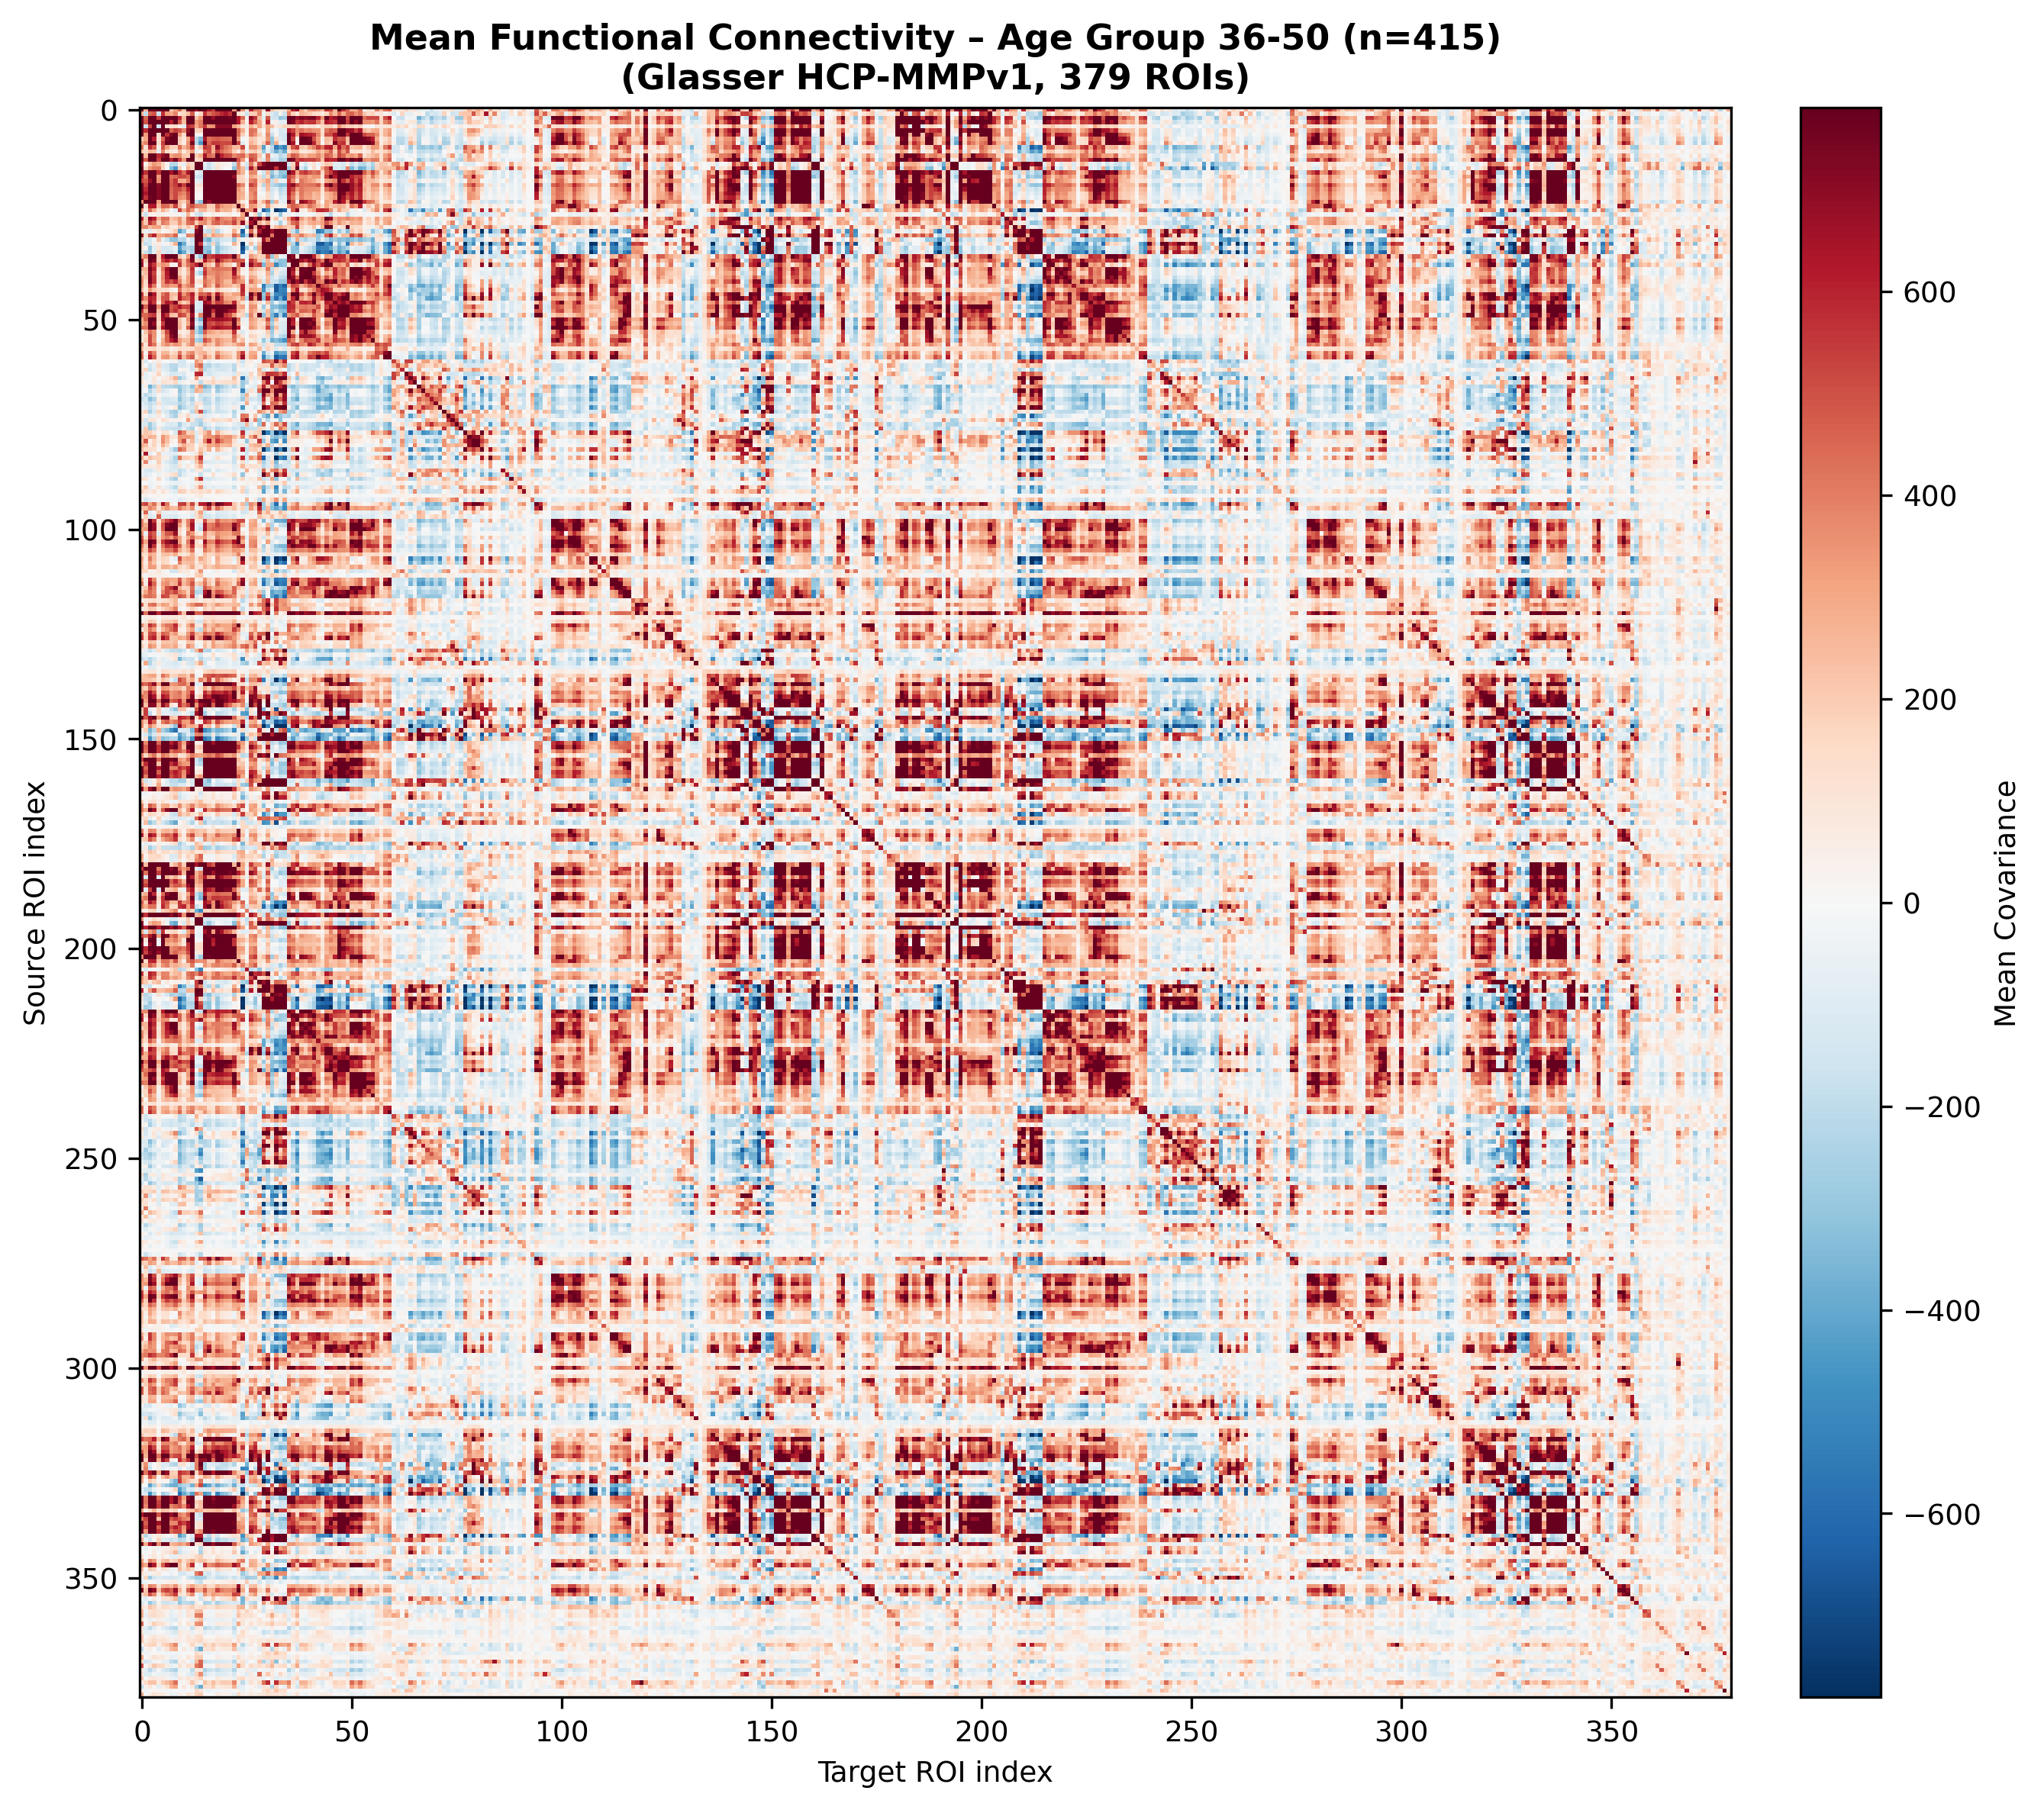
\includegraphics[width=\linewidth]{figures/heatmap_group_36_50.png}
        \caption{Age 36--50 (n=415)}
    \end{subfigure}
    \hfill
    \begin{subfigure}[b]{0.49\linewidth}
        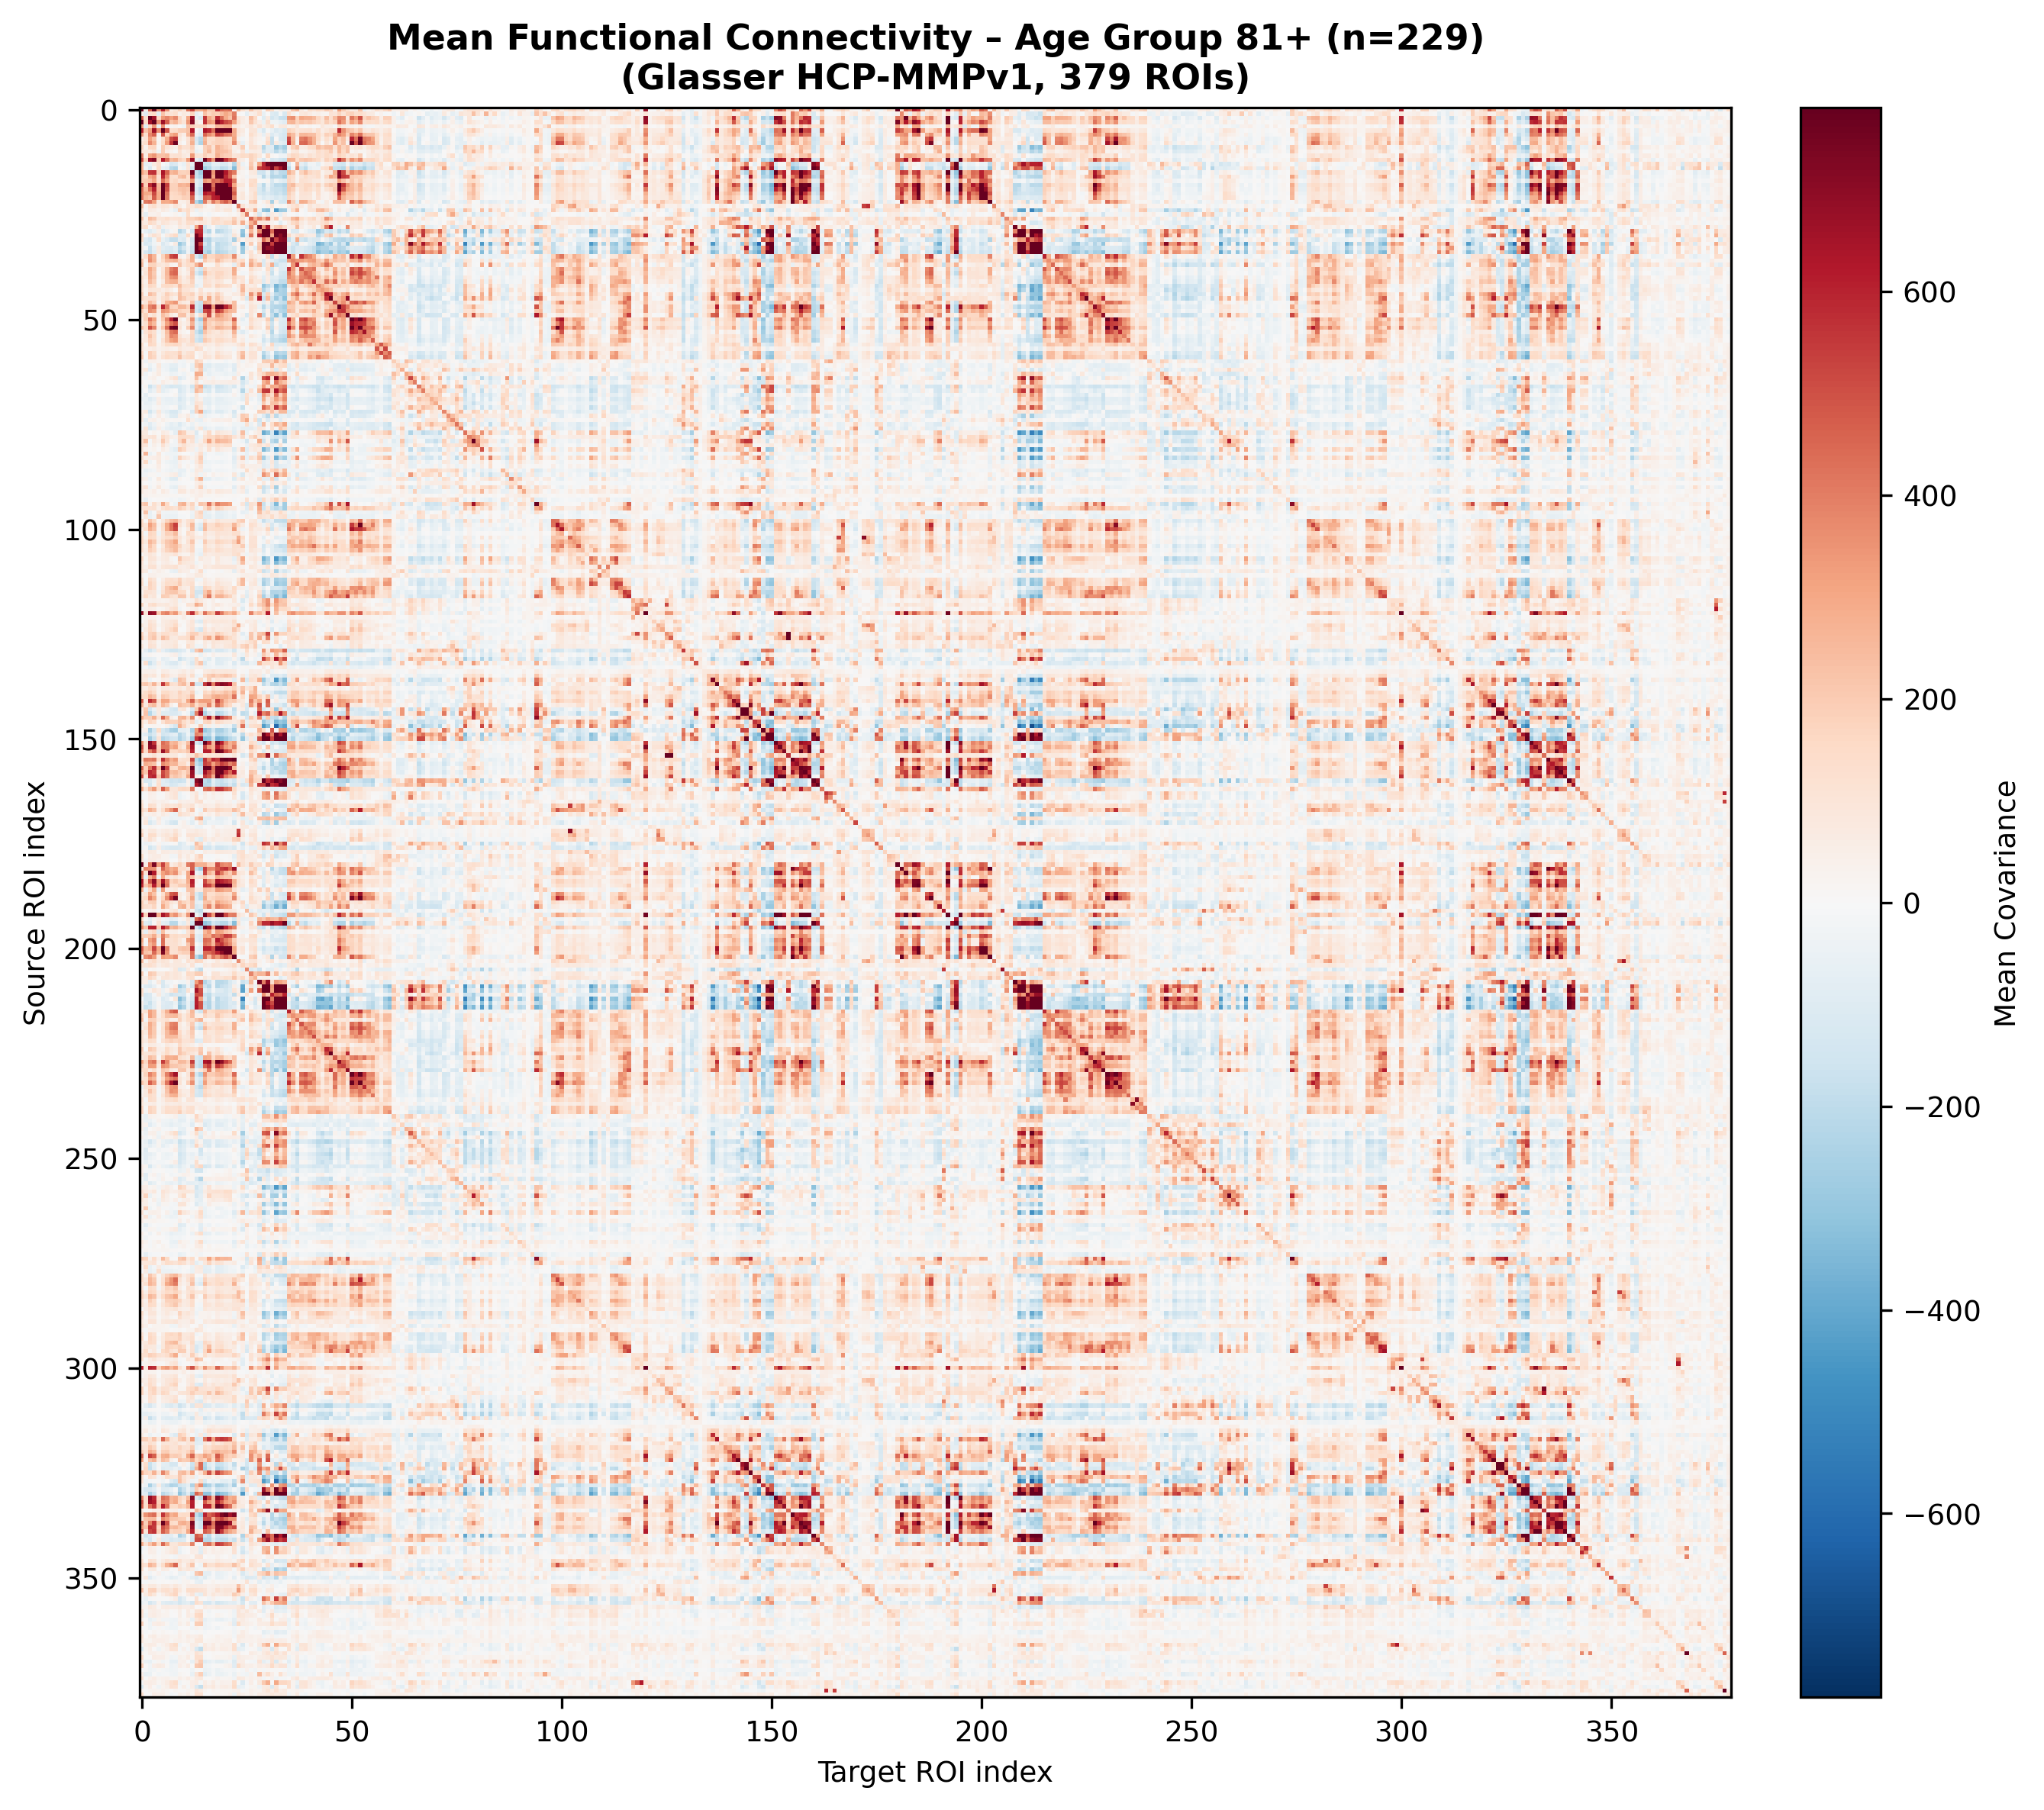
\includegraphics[width=\linewidth]{figures/heatmap_group_81plus.png}
        \caption{Age 81+ (n=229)}
    \end{subfigure}
    \caption{Mean covariance connectivity matrices for the youngest and oldest age groups (Glasser 379-ROI atlas, shared color scale).}
    \label{fig:groupmaps}
\end{figure}

\subsection{ANOVA Results}

One-way ANOVA across the four age groups was run at every edge (71,631 total). After FDR correction (Benjamini-Hochberg, q $<$ 0.05), \textbf{57,358 of 71,631 edges (80.1\%)} were significant, indicating that aging broadly affects the entire connectivity profile rather than isolated circuits.

Table~\ref{tab:anova} lists the top networks by mean F-statistic. Posterior Multimodal and Language networks show the strongest age effects, while the Default Mode Network shows the weakest among all named networks. The bar plot in Figure~\ref{fig:barplot} shows that every network follows a monotonic decrease in mean covariance from age 36 to 81+, with the Frontoparietal network showing the steepest absolute decline (approximately 70\%). The relative preservation of the DMN is consistent with prior literature showing that posterior cingulate and medial prefrontal hubs are among the last regions to lose connectivity in aging.

\begin{table}[h]
\centering
\small
\caption{Top networks by mean ANOVA F-statistic across age groups.}
\label{tab:anova}
\begin{tabular}{lc}
\toprule
\textbf{Network} & \textbf{Mean F} \\
\midrule
Posterior Multimodal  & 33.71 \\
Language              & 31.05 \\
Frontoparietal        & 29.23 \\
Cingulo-Opercular     & 28.04 \\
Subcortical           & 26.52 \\
Dorsal Attention      & 24.99 \\
Auditory              & 19.65 \\
Default Mode          & 16.36 \\
\bottomrule
\end{tabular}
\end{table}

\begin{figure}[h]
    \centering
    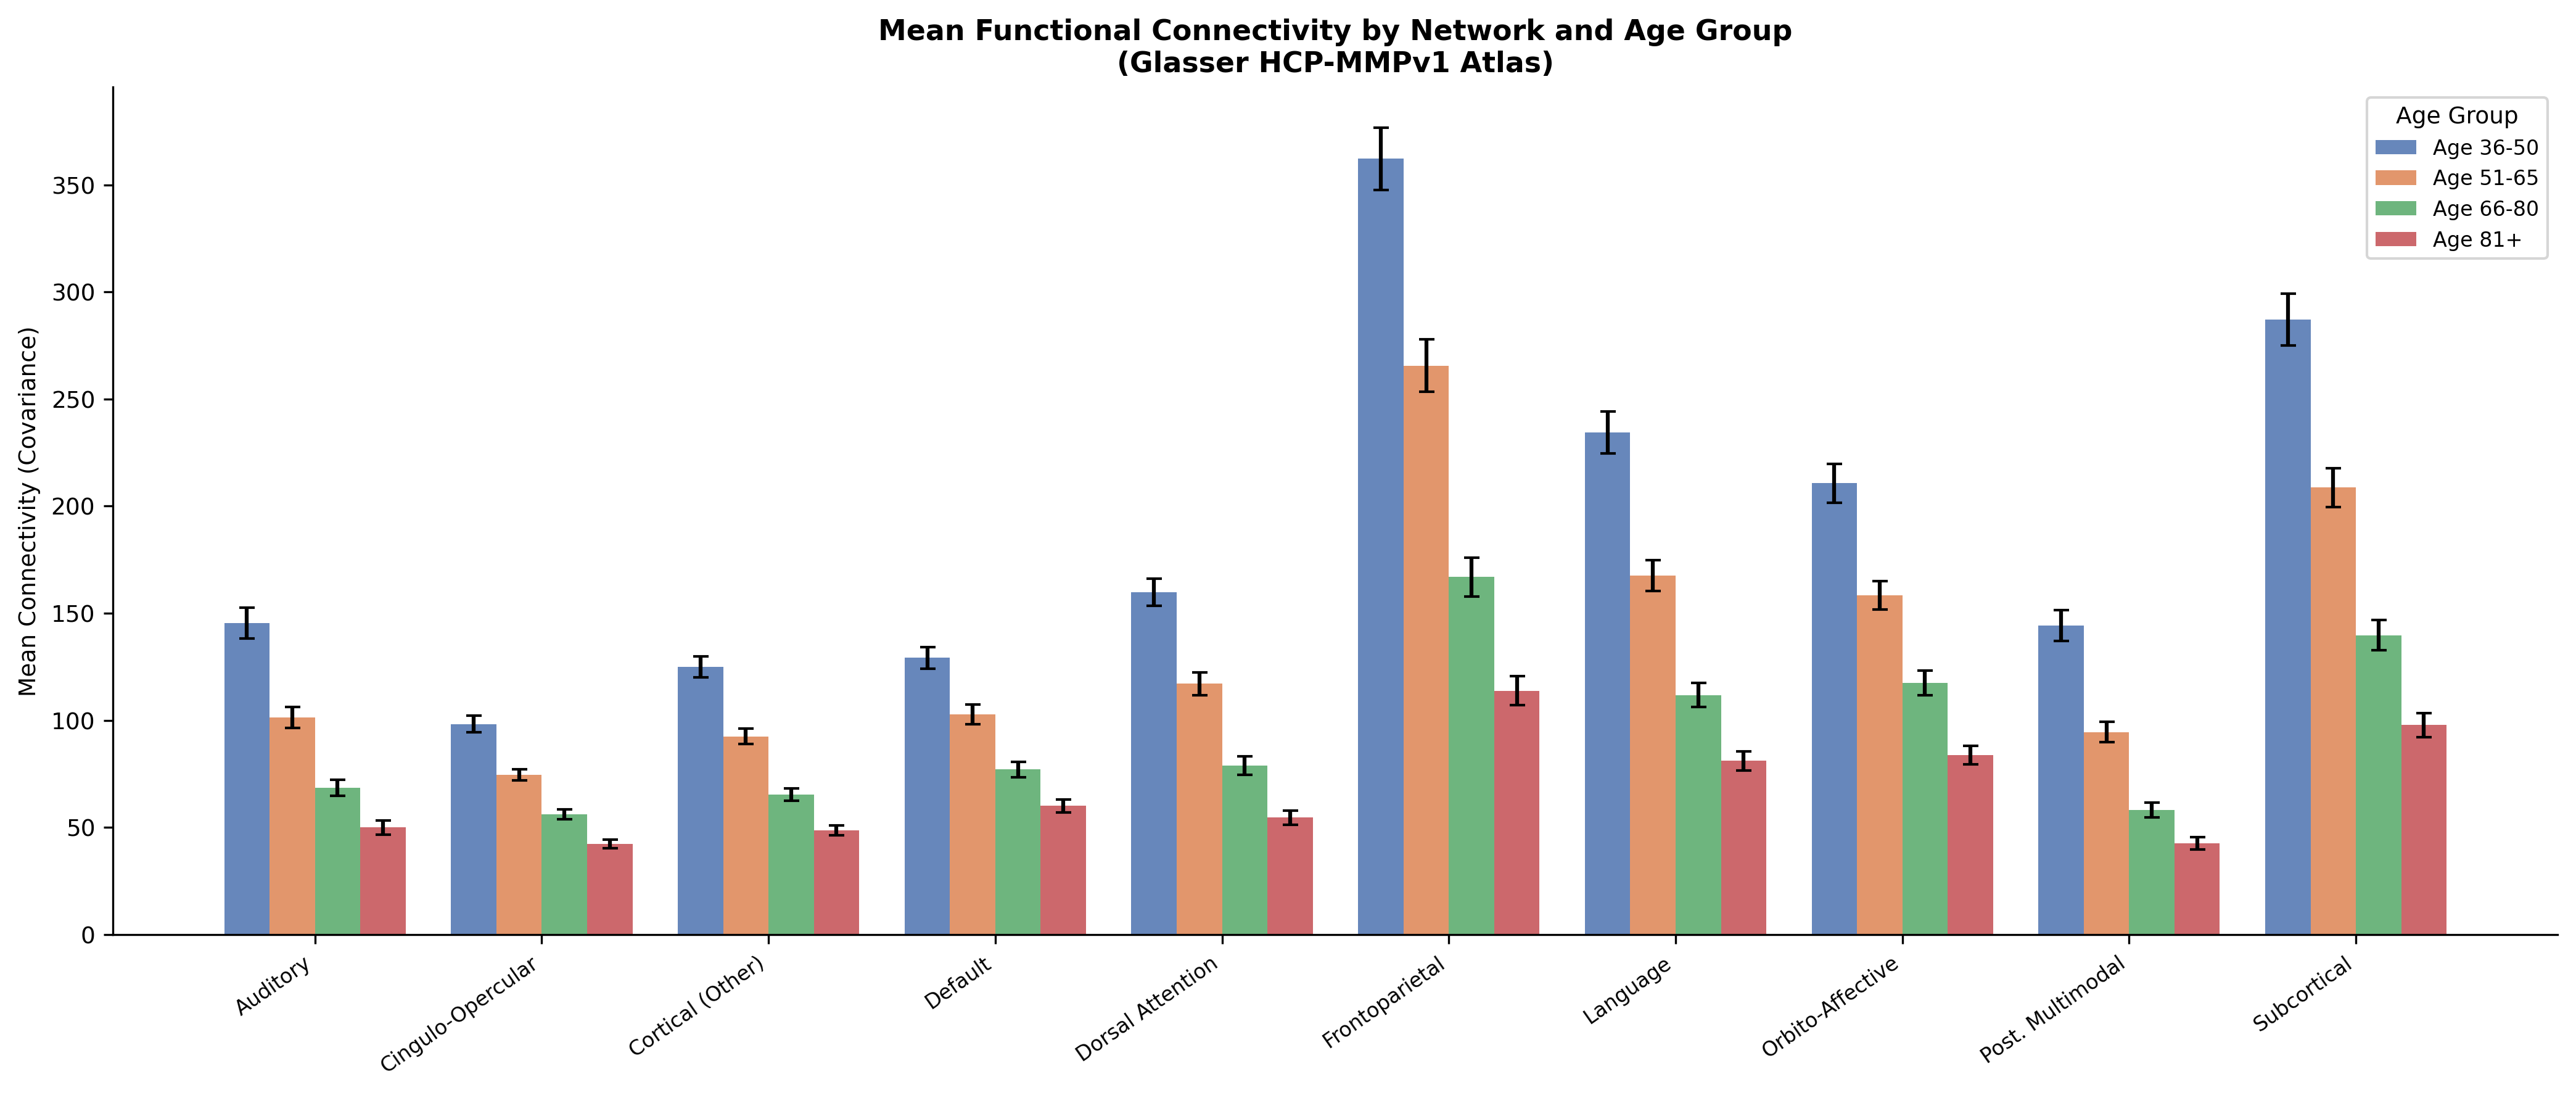
\includegraphics[width=\linewidth]{figures/network_contrast_barplot.png}
    \caption{Mean connectivity (covariance) per network across four age groups. Error bars show $\pm$1 SEM. All networks show monotonic decline with age.}
    \label{fig:barplot}
\end{figure}

% ============================================================
\section{Part 3: Connectome-Based Predictive Modeling}
% ============================================================

\subsection{Setup and Protocol}

CPM (Shen et al., 2017) was applied to predict \texttt{FluidIQ\_Tr35\_60y} from the 379-ROI covariance matrices using leave-one-out cross-validation (LOOCV) across 1,290 subjects with valid scores. At each fold, edges were selected via Pearson correlation with FluidIQ on N$-$1 training subjects (threshold: p $<$ 0.01), yielding positive (r $>$ 0) and negative (r $<$ 0) networks. Network strength was summed per subject and a linear model fitted on training subjects to predict the held-out subject.

\subsection{Results}

\begin{table}[h]
\centering
\small
\caption{CPM prediction performance for FluidIQ (LOOCV, n=1290).}
\label{tab:cpm}
\begin{tabular}{lccc}
\toprule
\textbf{Network} & \textbf{Pearson r} & \textbf{Spearman $\rho$} & \textbf{MAE} \\
\midrule
Positive          & 0.240** & 0.343 & 0.83 \\
Negative          & 0.333** & 0.360 & 0.80 \\
Combined (P$-$N)  & 0.283** & 0.368 & 0.81 \\
\bottomrule
\multicolumn{4}{l}{\small ** p $<$ 0.0001}
\end{tabular}
\end{table}

All three models achieve significant out-of-sample prediction (Table~\ref{tab:cpm}). The negative network (r = 0.333) outperforms the positive network, meaning that edges \textit{inversely} related to FluidIQ carry more predictive information. These edges likely represent connections between the Default Mode and task-positive systems; higher connectivity across these inter-network boundaries is associated with lower fluid intelligence, which aligns with the idea that individuals with greater cognitive capacity are better at segregating task-relevant and task-irrelevant circuits during rest.

Figure~\ref{fig:cpm} shows the predicted vs. observed scatter for all three models. The positive linear trend is clear in each panel, though considerable scatter is present -- the models explain roughly 6--11\% of variance in FluidIQ (r$^2$). Predictions are compressed toward the mean relative to observed scores, a standard feature of linear LOOCV regression. These effect sizes are consistent with published CPM results for fluid intelligence in single-cohort samples (Finn et al., 2015; Rosenberg et al., 2016). The wider age range of the AABC dataset introduces additional between-subject variance that likely limits predictive accuracy compared to more age-homogeneous studies.

\begin{figure}[h]
    \centering
    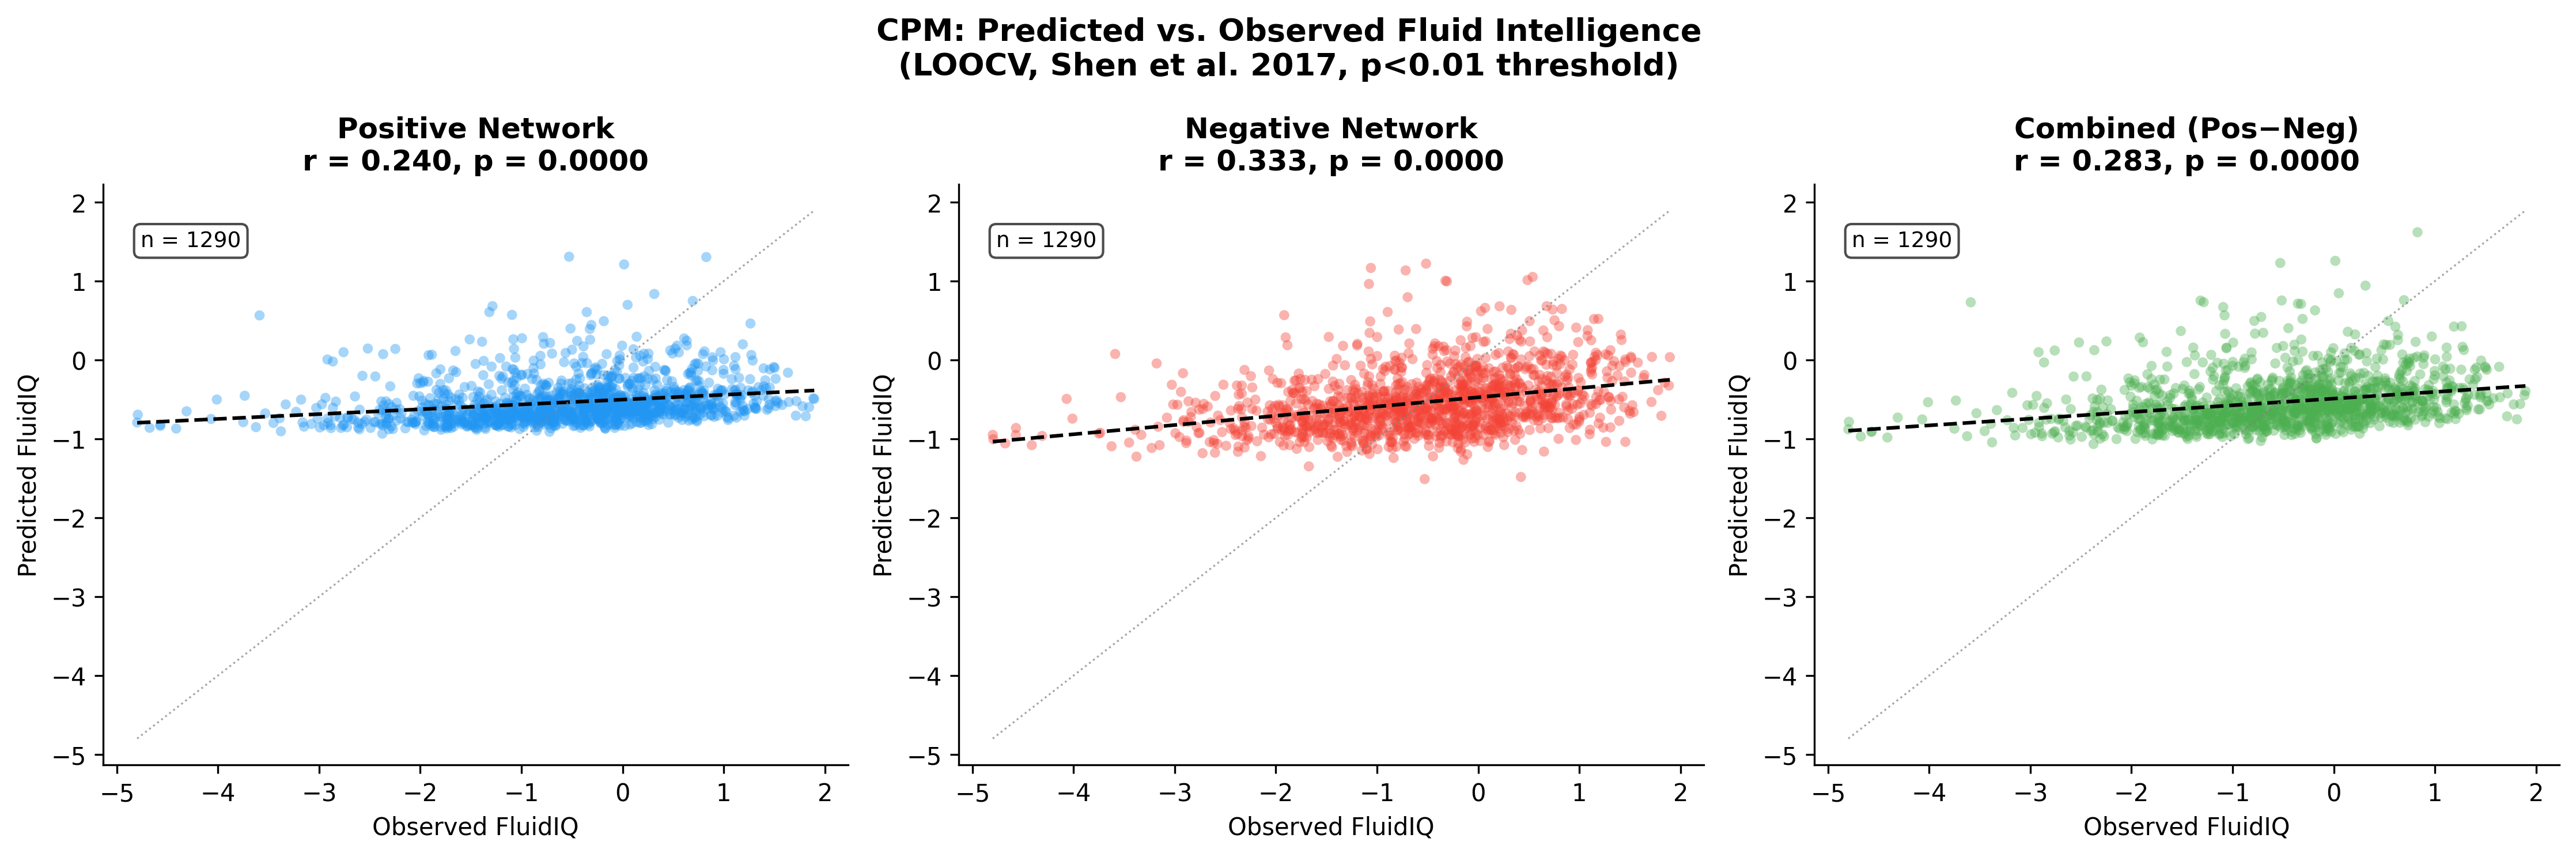
\includegraphics[width=\linewidth]{figures/scatter_predicted_vs_observed.png}
    \caption{CPM predicted vs. observed FluidIQ for positive (left), negative (center), and combined (right) networks. Dashed line shows the linear regression fit; dotted line shows the identity. Pearson r and p-value are annotated per panel.}
    \label{fig:cpm}
\end{figure}

% ============================================================
\section{Conclusion}
% ============================================================

This work demonstrated three findings. First, resting-state fMRI from a single HCP subject yields a well-structured 400-parcel connectivity matrix with clear network organization consistent with established resting-state literature. Second, aging in a large lifespan sample (n=1,390) produces broad, near-global reductions in functional connectivity, with association networks (Frontoparietal, Language, Posterior Multimodal) declining the most and the Default Mode Network showing relative preservation. Third, individual differences in fluid intelligence can be predicted from resting-state connectivity using CPM (best r = 0.333), with the negative network -- edges whose strength is inversely related to IQ -- providing stronger predictions than the positive network.

\begin{thebibliography}{9}
\small
\bibitem{park2009} Park, D.C., \& Reuter-Lorenz, P. (2009). The adaptive brain: aging and neurocognitive scaffolding. \textit{Annual Review of Psychology}, 60, 173--196.
\bibitem{finn2015} Finn, E.S., et al. (2015). Functional connectome fingerprinting: identifying individuals using patterns of brain connectivity. \textit{Nature Neuroscience}, 18, 1664--1671.
\bibitem{shen2017} Shen, X., et al. (2017). Using connectome-based predictive modeling to predict individual behavior from brain connectivity. \textit{Nature Protocols}, 12, 506--518.
\bibitem{fox2005} Fox, M.D., et al. (2005). The human brain is intrinsically organized into dynamic, anticorrelated functional networks. \textit{PNAS}, 102, 9673--9678.
\end{thebibliography}

\end{document}
